\documentclass[10pt]{article}
\usepackage[margin=0.85in]{geometry}
\usepackage{amsmath,amssymb,amsthm}
\usepackage{graphicx,booktabs,microtype}
\usepackage[font=small,labelfont=bf]{caption}
\usepackage[colorlinks=true,linkcolor=black,citecolor=black,urlcolor=blue]{hyperref}
\newtheorem{proposition}{Proposition}
\newcommand{\E}{\mathbb{E}}
\setlength{\parskip}{2pt}
\setlength{\textfloatsep}{8pt plus 2pt minus 2pt}\setlength{\intextsep}{8pt plus 2pt minus 2pt}

\title{How Much Is an AI Forecast Worth When Sales Are Censored?\\[2pt]
\large A pilot study of the robust newsvendor with a weak shadow variable}
\author{Tanishq Sahu\\ {\small BITS Pilani, K.K.\ Birla Goa Campus}}
\date{{\small Draft, November 2026 \quad$\cdot$\quad Code: \href{https://github.com/saint-broseph/censored-newsvendor-pilot}{\texttt{github.com/saint-broseph/censored-newsvendor-pilot}}}}

\begin{document}
\maketitle

\begin{abstract}
\noindent When a store runs out of stock, sales stop at the shelf count and the demand above it is lost. If stockouts are frequent enough, the optimal order quantity cannot be learned from sales at all, and a robust order must hedge against the worst demand the data allow. We ask how much a coarse, noisy AI demand forecast, used as a \emph{weak shadow variable} in the sense of Chen, Simchi-Levi and Xiong~\cite{csx}, is worth in this setting. We write the minimax-regret order under the forecast's constraints as a single linear program via LP duality, and verify it against the closed form of Hssaine and Sinclair~\cite{hs} (error $<10^{-13}$) and against brute force. On synthetic data with a critical ratio of 0.8, a five-level forecast cuts the excess cost of the robust order from 28\% to 0.26\% of the optimal cost and its guaranteed worst case from 97\% to 7.8\%. With everything estimated from 1{,}000 periods, the median excess cost is 0.6\%. The value persists until forecast noise exceeds the spread of demand. A forecast that under-predicts high demand, a bias invisible in uncensored data, can break the guarantee; a small relaxation restores it but does not remove the bias in the order.
\end{abstract}

\section{Question}
A newsvendor orders $q$ before demand $D\in\{0,\dots,M\}$ is seen, paying $b$ per unit short and $h$ per unit left over; the optimal order is the $\rho$-quantile of $D$, $\rho=b/(b+h)$. Past orders censor demand: we observe sales $\min(D,q)$ and whether a stockout occurred. With $\lambda$ the largest past order (the \emph{observable boundary}), sales identify $P(D=y)$ for $y<\lambda$ and the tail mass $m=P(D\ge\lambda)$, but nothing about how $m$ is spread over $\lambda,\dots,M$. Hssaine and Sinclair~\cite{hs} show that when $P(D<\lambda)<\rho$ the optimal order is not identified, and derive the minimax-regret order and its irreducible risk.

Retailers increasingly have a forecast from a pretrained model, seen in every period, including stockouts. Chen, Simchi-Levi and Xiong~\cite{csx} show that such predictions can tighten partial-identification bounds as extra linear constraints even when they are inaccurate. \textbf{How much does such a forecast shrink the ambiguity created by censoring, and how much inventory cost does it save?}

\section{Model}
\textbf{Signal.} The forecast is reported in $L$ buckets, like an LLM's 1--5 score: $F=\#\{c_k\le D+\mu+\sigma Z\}$ for cut points $c_1<\dots<c_{L-1}$ and $Z\sim N(0,1)$. Write $K_{fy}=P(F=f\mid D=y)$.

\textbf{Assumptions.} (A1) $F$ is independent of the stockout indicator given $D$; this holds when past orders do not depend on the forecast. (A2) The error model $K$ estimated where demand is observed ($y<\lambda$) also holds in the tail. A2 cannot be tested from censored data; Section~4.4 studies what happens when it fails.

\textbf{What the forecast adds.} In stockout periods at the largest order we observe $\beta_f=P(F=f,\,D\ge\lambda)$. Under A1--A2, $\sum_{y\ge\lambda}K_{fy}\,p_y=\beta_f$ for every $f$. The ambiguity set is
\begin{equation}
\mathcal{P}(\delta)=\Big\{p\ge 0:\ p_y=\hat p_y\ (y<\lambda),\ \textstyle\sum_{y\ge\lambda}p_y=m,\ \big\|K p_{\text{tail}}-\beta\big\|_1\le\delta\Big\}.
\end{equation}
$\delta=0$ trusts the error model exactly; $\delta>0$ allows for sampling error or misspecification; $\mathcal{P}(\infty)$ is the no-forecast set of~\cite{hs}.

\section{The robust order is one linear program}
With $c(q,y)=b(y-q)^++h(q-y)^+$ and $C_p(q)=\E_p\,c(q,D)$, the minimax-regret order solves
\begin{equation}
\min_{0\le q\le M}\ \max_{j\in\{0,\dots,M\}}\ \max_{p\in\mathcal{P}(\delta)}\ \big[C_p(q)-C_p(j)\big].
\end{equation}
Benchmarking against integer orders $j$ is exact because $C_p$ is piecewise linear with integer breakpoints.

\begin{proposition}
Problem (2) equals the linear program
\begin{align*}
\min\ t\quad\text{s.t.}\quad
&\textstyle\sum_{y<\lambda}\hat p_y\,(z_y-c(j,y)) + m\,\mu_j+\beta^\top(\nu^+_j-\nu^-_j)+\delta\,\eta_j\le t, && j=0,\dots,M,\\
&\mu_j+[K^\top(\nu^+_j-\nu^-_j)]_y\ \ge\ b(y-q)-c(j,y), && y\ge\lambda,\ \forall j,\\
&\mu_j+[K^\top(\nu^+_j-\nu^-_j)]_y\ \ge\ h(q-y)-c(j,y), && y\ge\lambda,\ \forall j,\\
&\nu^+_{jf}+\nu^-_{jf}\le\eta_j,\quad z_y\ge b(y-q),\quad z_y\ge h(q-y)\ (y<\lambda),\quad \nu,\eta\ge0,\quad 0\le q\le M.
\end{align*}
\end{proposition}
\noindent\emph{Proof sketch.} For fixed $q$ and $j$ the inner maximisation over $p$ is a feasible, bounded LP; by strong duality~\cite{bt} it equals its dual, a minimisation over $(\mu_j,\nu_j^\pm,\eta_j)$. Replacing each inner max by its dual turns ``$\min_q\max_j$'' into one minimisation. The dual constraints contain $c(q,y)$, the maximum of two functions affine in $q$, which splits into the two linear inequalities shown; the known part of the cost uses the epigraph variables $z_y$. $\square$

Without the forecast (no $\nu,\eta$), the LP must reproduce the closed form of~\cite{hs}. It does, to $2\times10^{-14}$ in all 20 unidentifiable cases of a grid over $\lambda$ and $(b,h)$, and returns zero regret in the 5 identifiable ones (experiment E1). The test suite (26 tests) also checks that the LP value equals the worst case found by solving every inner primal LP directly, that no other order does better, that the worst-case distribution lies in $\mathcal{P}(\delta)$, and that the Kaplan--Meier and error-model estimators recover known truths.

\section{Experiments}
\textbf{Setup.} $M=80$; demand is negative binomial with mean 30 and s.d.\ 13.1; $b=4$, $h=1$, so $\rho=0.8$ and $q^*=40$ with optimal expected cost $C^*=20.13$. Past orders are 26, 30 and 34 in equal shares, so $\lambda=34$ and $P(D<\lambda)=0.65<\rho$: the optimal order is not identified. The main forecast has $L=5$ buckets (cuts at 20, 30, 40, 50) and noise $\sigma=4$. We report \emph{excess cost}, the regret as a share of $C^*$, both \emph{actual} (under the true demand) and \emph{guaranteed} (the LP's worst case). Infinite-data experiments relax $\delta$ by the sampling error of $n=1{,}000$ periods, $\delta=m\sqrt{L/n_s}$ with $n_s$ the expected number of stockouts at $\lambda$.

\begin{figure}[!htb]
\centering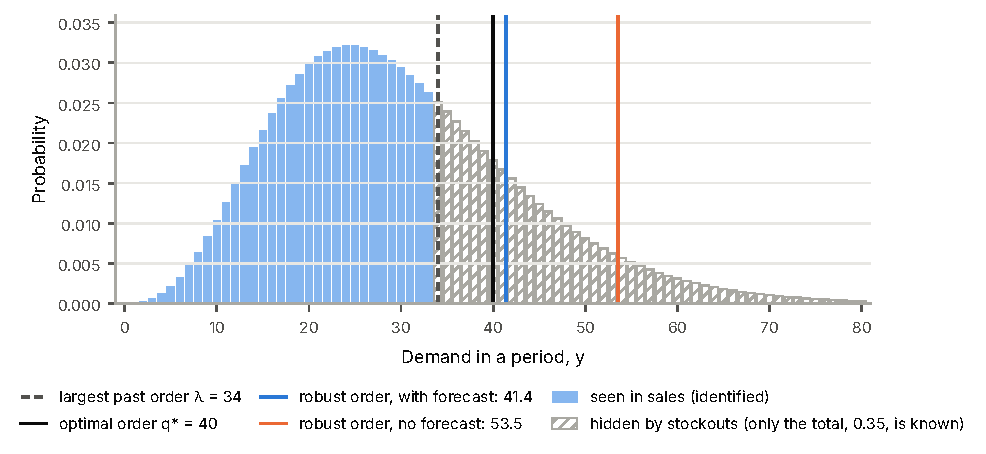
\includegraphics[width=0.82\textwidth]{../figures/fig1_setup.pdf}
\caption{Demand above $\lambda=34$ is hidden by stockouts. Without a forecast the robust order hedges against demand as high as 80 and orders 53.5; with the five-level forecast it orders 41.4, close to $q^*=40$.}
\end{figure}

\subsection{A coarse forecast removes almost all of the cost of censoring}
Without the forecast, the robust order is 53.5 (Fig.~1): its guaranteed worst case is 97\% excess cost and its actual excess cost is 28.0\%. Treating sales as demand orders 30 and does no better (28.6\%). With the five-level forecast at $\sigma=4$ the order is 41.4, the guarantee falls to 7.8\% and the actual excess cost to 0.26\%: \textbf{99.1\% of the cost of censoring is recovered}. Figure~2 shows the value persisting until the noise reaches about the spread of demand ($\sigma/\text{sd}\approx1$) and then decaying; at $\sigma=128$ the five-level forecast recovers 11\%, and at $\sigma=256$ nothing.

Two details are worth noting. First, more buckets help only while the forecast is sharp: each bucket is estimated from fewer stockouts, so the allowance grows with $\sqrt{L}$ and fine forecasts lose value sooner once noisy. Second, a binary forecast with a hard cut ($\sigma=0$) recovers only 77\%: it says demand is above 40 but not how far. A little noise spreads that information across the tail and helps (0.07\% excess cost at $\sigma=16$).

\emph{A caution about infinite data.} With $\delta=0$ and an exactly known error model, even a nearly pure-noise forecast ($\sigma=256$) keeps the guarantee at 5.6\%, because a known smooth kernel still reveals averages of the tail. That information vanishes under realistic sampling error, echoing the ill-conditioning of weak shadow variables noted in~\cite{csx}. This is why every infinite-data result here includes a sampling allowance.

\begin{figure}[!htb]
\centering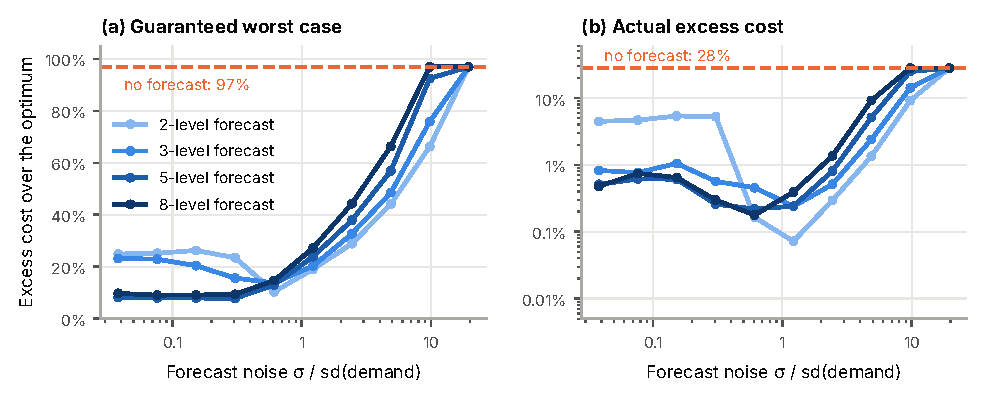
\includegraphics[width=0.86\textwidth]{../figures/fig2_value_vs_noise.pdf}
\caption{Value of the forecast against its noise, for 2--8 buckets, with a sampling allowance for 1{,}000 periods. Dashed: no forecast. (a) The guaranteed worst case stays near 8--25\% until noise exceeds the demand spread. (b) With three or more levels, actual excess cost stays at or below about 1\% until the noise exceeds the demand spread.}
\end{figure}

\subsection{The heavier the censoring, the more the forecast is worth}
Moving the boundary from $\lambda=40$ ($P(D<\lambda)=0.79$) down to $\lambda=20$ ($0.23$) raises the actual excess cost of the no-forecast robust order from 1.2\% to 74\%, and of the sales-as-demand order from 6.9\% to 128\% (Fig.~3). With the forecast it stays below 0.4\% throughout, and its guarantee rises only from 3.2\% to 14\%, against 14\% to 221\% without it.

\begin{figure}[!htb]
\centering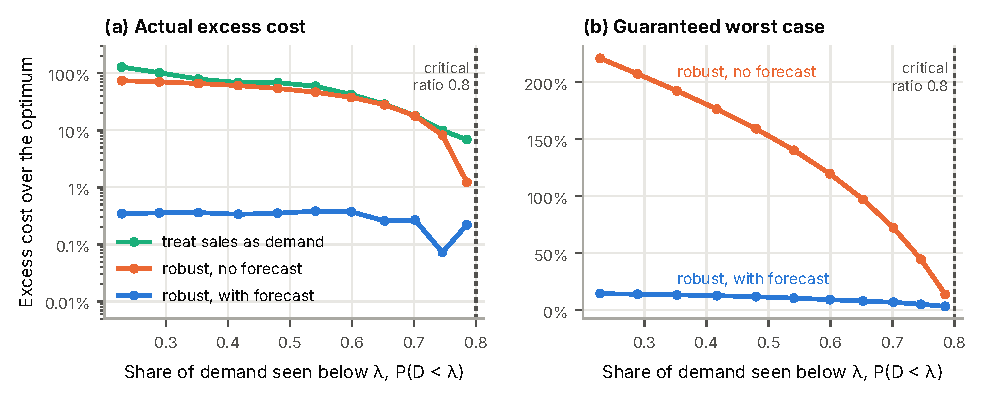
\includegraphics[width=0.86\textwidth]{../figures/fig3_value_vs_censoring.pdf}
\caption{Value of the forecast against the severity of censoring. Left of the dotted line the optimal order is not identified from sales.}
\end{figure}

\subsection{When the error model is wrong}
A forecaster trained on censored sales may under-predict high demand. We let the forecast's centre be $D-\kappa(D-\lambda)^+$ while the analyst keeps assuming $\kappa=0$. Because the bias is zero below $\lambda$, it is invisible in the uncensored periods used to fit the error model (Fig.~4). With $\kappa=0.3$ the order is 38.8 and the guarantee holds at every $\delta$. With $\kappa=0.6$, \textbf{at $\delta=0$ the guarantee is broken}: it claims 0.8\% excess cost while the actual is 3.4\%. A relaxation of $\delta\ge0.005$ restores a valid guarantee, long before the true distribution itself re-enters the set ($\delta^*=0.19$). But the order stays between 36.5 and 37.1 for every $\delta\le0.2$: relaxing the constraints repairs the guarantee, not the bias.

\begin{figure}[!htb]
\centering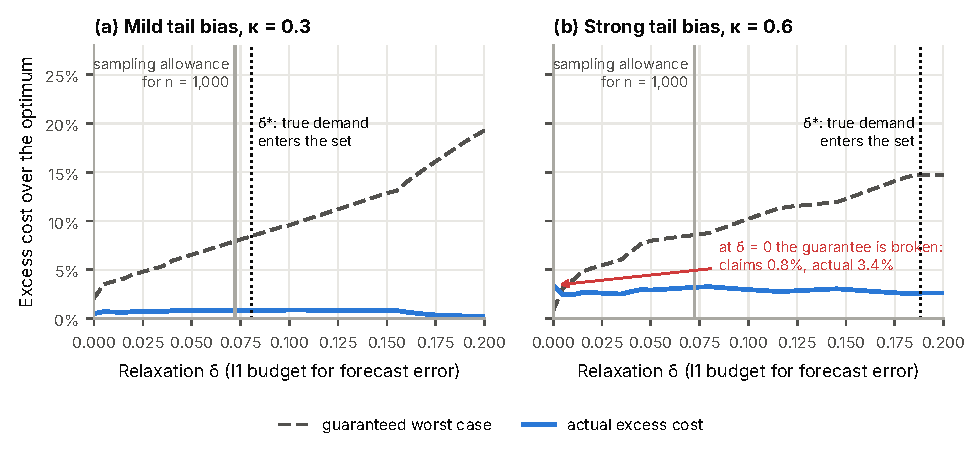
\includegraphics[width=0.86\textwidth]{../figures/fig4_misspecification.pdf}
\caption{A forecast that under-predicts demand above $\lambda$ by a fraction $\kappa$. Grey line: the sampling allowance for 1{,}000 periods; dotted line: the $\delta$ at which the true distribution enters the set.}
\end{figure}

\subsection{Everything estimated from data}
Finally we simulate $n$ periods, estimate $\hat p_y$ and $m$ by Kaplan--Meier~\cite{km,huh}, fit $(\mu,\sigma)$ by maximum likelihood on uncensored periods, set $\delta=m\sqrt{L/n_s}$ (raised if needed to keep the set non-empty), and solve the LP; 100 replications per cell (Fig.~5). With $\sigma=4$ the median excess cost is 1.6\% at $n=250$, 0.61\% at $n=1{,}000$ and 0.08\% at $n=4{,}000$, while both alternatives stay near 28\%. The guarantee held in every run except 5 of 100 at $\sigma=16$, $n=250$.

\begin{figure}[!htb]
\centering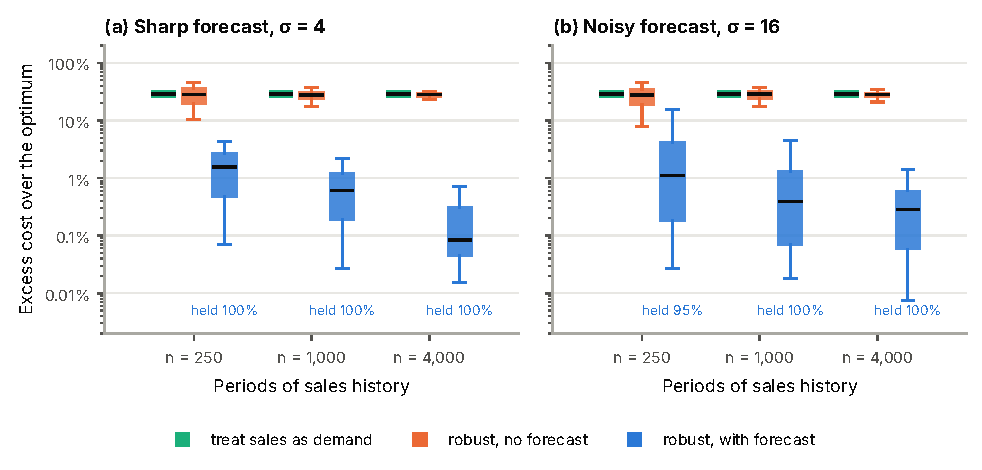
\includegraphics[width=0.86\textwidth]{../figures/fig5_finite_sample.pdf}
\caption{Excess cost with all inputs estimated from $n$ simulated periods (boxes: quartiles; whiskers: 5th--95th percentiles; 100 replications). ``Held'': share of runs in which the guarantee was at least the actual excess cost.}
\end{figure}

\section{Limitations and next steps}
\begin{itemize}\setlength{\itemsep}{1pt}
\item \textbf{Inference.} The allowance $\delta=m\sqrt{L/n_s}$ is a heuristic with no coverage guarantee. Chen et al.~\cite{csx} use an $\ell_1$-penalised LP with a data-driven radius and recentred subsampling for valid confidence intervals; implementing that is the natural next step.
\item \textbf{A2 cannot be tested.} Section~4.4 shows it matters. A sensitivity model on the response odds, as in~\cite{csx}, may describe forecast error more realistically than an $\ell_1$ budget.
\item \textbf{A1 fails under feedback.} If past orders were set from the forecast, a stockout depends on $F$ given $D$ and the exclusion condition fails by construction. How to bound that case is an open question I would like to study.
\item \textbf{Scope.} Synthetic data, one product, no covariates, a single period; the no-forecast hedge depends on the support bound $M$. A stockout-annotated retail dataset would be the first real-data test.
\end{itemize}

\begin{thebibliography}{9}\small
\bibitem{csx} H.~Chen, D.~Simchi-Levi, R.~Xiong. Partial identification under missing data using weak shadow variables from pretrained models. arXiv:2602.16061, 2026.
\bibitem{hs} C.~Hssaine, S.~R.~Sinclair. The data-driven censored newsvendor problem. arXiv:2412.01763, 2024.
\bibitem{bsw} J.~Bu, D.~Simchi-Levi, L.~Wang. Offline pricing and demand learning with censored data. \emph{Management Science} 69(2), 2023.
\bibitem{bt} D.~Bertsimas, J.~N.~Tsitsiklis. \emph{Introduction to Linear Optimization}. Athena Scientific, 1997.
\bibitem{km} E.~L.~Kaplan, P.~Meier. Nonparametric estimation from incomplete observations. \emph{J.\ American Statistical Association} 53(282):457--481, 1958.
\bibitem{huh} W.~T.~Huh, R.~Levi, P.~Rusmevichientong, J.~B.~Orlin. Adaptive data-driven inventory control with censored demand based on Kaplan--Meier estimator. \emph{Operations Research} 59(4):929--941, 2011.
\end{thebibliography}
\end{document}
